\documentclass[draft,10pt,twocolumn,letterpaper]{article}

\usepackage{cvpr}
\usepackage{times}
\usepackage{epsfig}
\usepackage{graphicx}
\usepackage{amsmath}
\usepackage{amssymb}
\usepackage{graphicx} % Allows you to include images
\usepackage{enumitem} % Allows customization of list spacing
\usepackage{float} % To control float positioning
\usepackage{placeins} % For FloatBarrier
\usepackage{booktabs}
\usepackage{multirow}
\usepackage{afterpage}
\usepackage{amssymb}

% Include other packages here, before hyperref.

% If you comment hyperref and then uncomment it, you should delete
% egpaper.aux before re-running latex.  (Or just hit 'q' on the first latex
% run, let it finish, and you should be clear).
\usepackage[pagebackref=true,breaklinks=true,letterpaper=true,colorlinks,bookmarks=false]{hyperref}

\cvprfinalcopy % *** Uncomment this line for the final submission

\def\cvprPaperID{****} % *** Enter the CVPR Paper ID here
\def\httilde{\mbox{\tt\raisebox{-.5ex}{\symbol{126}}}}

% Pages are numbered in submission mode, and unnumbered in camera-ready
%\ifcvprfinal\pagestyle{empty}\fi
\begin{document}

%%%%%%%%% TITLE
\title{Project Report : CS 7643}

\author{Girish Sharma\\
{\tt\small gsharma@gatech.edu}
% For a paper whose authors are all at the same institution,
% omit the following lines up until the closing ``}''.
% Additional authors and addresses can be added with ``\and'',
% just like the second author.
% To save space, use either the email address or home page, not both
\and
Matias Vizcaino \\
{\tt\small avizcaino3@gatech.edu}
\and
William Gleason\\
{\tt\small wgleason3@gatech.edu}
}

\maketitle
%\thispagestyle{empty}

%%%%%%%%% ABSTRACT
\begin{abstract}
   We evaluate adapters as a parameter efficient alternative to fine-tuning a model for a given task. We first fine-tune a pre-trained model to perform a given task and then use the same pre-trained model to introduce adapter modules and perform the same task using an adapter-based approach. We see that adapters can achieve comparable performance to fine-tuning. A similar observation can be made even when the model undergoes a second-phase of task-adaptive pre-training before fine-tuning. Beyond comparable performance, adapters have significant benefits over fine-tuning, in terms of greatly reduced trainable parameters, ability to perform sequential training on tasks, and combining multiple adapters to create a single model capable of performing multiple tasks.
\end{abstract}

%%%%%%%%% BODY TEXT
\section{Introduction/Background/Motivation}

\subsection{Objective} We explore how traditional methods using fine-tuning compare to newer architectures using adapters in the context of transfer learning with pre-trained models for natural language tasks. We conduct a comparison across 4 types of pre-trained models that have been used before in other studies \cite{gururangan2020dont}. 1. A generic LLM, RoBERTa. 2. An LLM pre-trained on text in the domain of a task (DAPT). 3. An LLM pre-trained on the unlabeled data from a specific task (TAPT) 4. LLM pre-trained on both (DAPT + TAPT). 

Adapters are more lightweight, modular and composable than traditional fine-tuning methods. However, there may exist a performance penalty due to the reduced number of trainable parameters. This project looks at using parameter-efficient adapters for the RoBERTa transformer to achieve comparable performance to fine-tuning. Expanding from (Houlsby et al., 2019), our scope consists of two adapter configurations (Pfeiffer and Houlsby) imposed over tasks that contain specialized language and domains not extensively available in the base RoBERTa model. This allows us to assess if adapters can infuse knowledge efficiently, in a way that is comparable to Gururangan’s Task Adaptive Pretraining (TAPT) with small datasets related to two tasks in the Computer Science domain and one task for Biomedicine. Additionally, we evaluate the effectiveness of Adapter Fusion, a recently proposed multi-task learning architecture that aims to leverage multiple modular adapters using an attention layer. 

Throughout the study, we evaluate our models and compare them by the F1-Macro Score and the number of trainable parameters of their network, with specific focus on traditional fine-tuning, TAPT pre-training, and adapter methods. Albeit we focus on a small number of low-resource tasks ($<$ 5K records), the results support the potential of adapters as a parameter-efficient contestant to fine-tuning and as a viable alternative to TAPT for some use-cases, such as mid-sized ($>$ 3K) datasets.

\subsection{Current State} A common practice today is to start with a model pre-trained on a broad corpus of information (such as books, websites and other general domains) and then use fine-tuning to train the model for a particular task. If the task sits within a specific domain not originally covered by model, continued  pre-training can be done on specific unlabelled corpus. Once a baseline pre-trained model has been established, task specific heads are added as the final layers, which get co-trained with the baseline weights using task specific labeled data. Fine-tuning has been shown to be very effective at performing a given task.
\begin{itemize}
\item \textbf{Pre-Trained Models} like RoBERTa, a bidirectional encoder model, uses techniques like Masked Language Modeling (MLM) and Next Sentence Prediction (NSP) to learn a deep understanding of language structure and continuity. An optional second phase of pre-training \cite{gururangan2020dont} continues the process on new data using the same unsupervised learning objectives. The internal weights and embeddings of the model are shifted to better represent the vocabulary and patterns found in the new data. These processes are often quite demanding in terms of data and compute resources.

\item \textbf{Full Fine-Tuning} is then used retrain the entire model on the task data. While this would likely lead to the best performance, studies have shown that earlier layers of the pre-trained model generally learn broad semantic and syntactic features and those don’t really change for any given task. Limitations of fine-tuning include the need to store and share a complete set of weights for each task, and the requirement to train all tasks simultaneously to avoid catastrophic forgetting \cite{mccloskey1989catastrophic}.

\item \textbf{Variable Fine-Tuning} arises as a more efficient way to fine-tune. Researchers have shown that Parameter-Efficient-Fine-Tuning (PEFT) methods that focus only on a small proportion of model weights (original or new), while keeping the remaining weights frozen, can match the performance of traditional full fine-tuning methods \cite{houlsby2019parameter} and address some of their limitations, largely as they preserve much of the original knowledge while still adapting to new tasks. 

\end{itemize}
\subsection{Motivation}  Fine-tuning has several benefits as it allows to use the learned representations of large pre-trained models for specific tasks. However, it also has some
drawbacks.

\begin{itemize}
    \item Fine-tuning involves training a large number of parameters for each task. For large models which can be 100s of MB, storing and sharing a complete set of weights for each task can limit multi-task applications.
    \item All tasks must be trained simultaneously. Sequential fine-tuning for multiple tasks leads to catastrophic forgetting \cite{mccloskey1989catastrophic}
\end{itemize}
Adapters do not suffer from these drawbacks \cite{houlsby2019parameter}. The number of trained parameters is a tiny fraction compared to fine-tuning, significantly reducing the computational resources for fine-tuning \ref{tab:model-parameters}. Additionally, adapters are modular as multiple adapters can be loaded onto the same base model to perform multiple tasks, eliminating the need for a copy of the base model for each task. Further, as they preserve the original model weights, they are more capable of maintaining the base model integrity and performance across tasks.

Gururangan et al. \cite{gururangan2020dont} highlights the benefits of domain-adaptive pre-training (DAPT) and task-adaptive pre-training (TAPT), which tailor the pre-training phase to more closely align with the characteristics of the target tasks, potentially enhancing subsequent fine-tuning outcomes. For instance, they expose low vocabulary overlap between RoBERTa and the domain of Computer Science, and find that continued pre-training on this domain is beneficial for related tasks. Their insights are crucial for informing more efficient strategies for effective task-specific tuning, although they rely on expensive methods of retraining and fine-tuning. In “Parameter-Efficient Transfer Learning for NLP” \cite{houlsby2019parameter}, the authors show that adapters attain within 0.4\% of the performance of full-fine-tuning, adding only 3.6\% parameters per task. The paper used the BERT transformer as its pre-trained model and used tasks from the GLUE benchmark to prove its assertions. 

We study parameter-efficient task adaptation using the RoBERTa model, which is a more robust version of BERT \cite{liu2019roberta}, and compare the results to those of \cite{gururangan2020dont}. As per \cite{houlsby2019parameter}, we expect the performance of adapters to be comparable to full fine-tuning, and further explore the capabilities for adapters as a viable alternative to TAPT to perform on out-of-domain tasks.

\begin{table*}[h]
  \centering
  
  \begin{tabular}{ l l l r r r r }
    \hline
    \textbf{Domain} & \textbf{Task} & \textbf{Label Type} & \textbf{Train} & \textbf{Dev}   & \textbf{Test}  & \textbf{Classes} \\
    \hline
    Computer Science & ACL-ARC & citation intent & 1,688 & 114   & 139   & 6 \\
                     & SCIERC  & relation classification & 3,219 & 455   & 974   & 7 \\
    \hline
    BIOMED           & CHEMPROT & relation classification & 4,169 & 2,427 & 3,469 & 13 \\
    \hline
  \end{tabular}%
  \caption{\textbf{Dataset Statistics}}
  \label{tab:dataset-stats}%
\end{table*}%


\begin{table*}[h]
    \centering
    
    \begin{tabular}{ l r r r }
        \hline
        \textbf{Model} & \textbf{Parameter Counts} & \textbf{Parameters Trained} & \textbf{Percentage Trained} \\
        \hline
        RoBERTa & 124,650,246 & 124,650,246 & 100.00\% \\
        Pfeiffer Adapters & 126,777,759 & 2,127,513 & 1.71\% \\
        Houlsby Adapters & 127,672,287 & 3,022,041 & 2.42\% \\
        \hline
    \end{tabular}
    \caption{\textbf{Model Parameters and Training Percentage}}
    \label{tab:model-parameters}
\end{table*}


%-------------------------------------------------------------------------
%------------------------------------------------------------------------
\section{Approach}
Our objective is to establish adapters as a suitable transfer learning approach for a given task, as compared with fine-tuning and task-adaptive pretraining methods. For this we recreate the baseline that was used in the transfer learning paper \cite{gururangan2020dont}. We then take the four pre-trained models (RoBERTa base, DAPT, TAPT, DAPT-TAPT) per task and train adapters under two configurations, Pfeiffer and Houlsby. Our results are directly comparable to the original paper \cite{gururangan2020dont} and our own reproduction of their results.

\subsection{Data, Domain, and Tasks} We take data available to download by Allen Institute \cite{allenai_dont_stop_pretraining}. Our scope \footnote{Attempts were made to train on high-resource tasks, but due to computational demands, this was infeasible within our timeframe and is set as a future objective. We further exclude the low-resource NEWS task HYPERPARTISIAN as the test/validation dataset is very small and has only 2 classes - this leads to inconsistent results from \cite{allenai_dont_stop_pretraining} under our current set-up, again to be investigated as a future objective.} is a subset of tasks from \cite{gururangan2020dont} that includes two tasks under the CS domain, ACL-ARC (citation-intent) and SCIERC (relation classification), and one task from BIOMED domain, CHEMPROT (relation classification) to test our hypothesis under a new domain. All these tasks have under 5,000 training records (i.e., low-resource). Table \ref{tab:dataset-stats}.

The task datasets show similar class distribution and are imbalanced \textcolor{blue}{[TODO - APPENDIX]}. Therefore, we use the F1 score as our evaluation metric, which is a better measure for imbalanced datasets. The F1 score is the harmonic mean of precision and recall, and is a better measure for imbalanced datasets. Also, this is the same metric used in the original paper \cite{gururangan2020dont} so it allows for comparison of results.

\subsection{Methodology} 

\textbf{Base Models and Fine-Tuning} For reproduction, we first aimed to use the same set-up as in \cite{allenai_dont_stop_pretraining} but encountered limitations on compatibility with newer packages and versioning. Therefore, we chose the widely used HuggingFace Transformers library \cite{transformers} for training our models. We load the pre-trained models from \cite{allenai_dont_stop_pretraining} available in HuggingFace, and fine-tune by training a classification head in supervised manner using the same task-specific datasets and approach \cite{gururangan2020dont}. We were able to recreate results that are close-enough to the reference paper (better in some cases), but further efforts may be needed for closer replication and inspection of original process \footnote{Although benchmark fine-tuning results broadly align, there are some differences, likely due to differences in infrastructure, libraries used, and possibly unreported training parameters. Biggest relative difference is our F1 roberta-base for ACL-ARC at 66.34 while Gururangan’s is 63.00}. The F1 metric from our version of fine-tuning results is taken as a benchmark to assess the performance of adapter methods.

\textbf{Adapters}  To assess the efficacy of adapter methods, for every task we add task-specific adapters (and a prediction head) to each of the base models and train them on the task-specific data. For training and managing adapters, we use AdapterHub’s library \cite{adapterhub_overview} and two of their adapter architectures: Pfeiffer \cite{pfeiffer2020adapterhub} a lightweight configuration that adds the adapter modules between the feed-forward layers, and Houlsby \cite{houlsby2019parameter} which can handle more complexity as it adds adapter modules between the multi-head attention layer. The APPENDIX \ref{sec:pfeiffermodel} \ref{sec:houlsbymodel} shows examples of the adapter modules added to the model for both configurations. We compare results under two scopes: direct fine-tuning comparison, and continued taks-adaptive pre-training comparison.


\begin{figure}[h]
    \centering 
    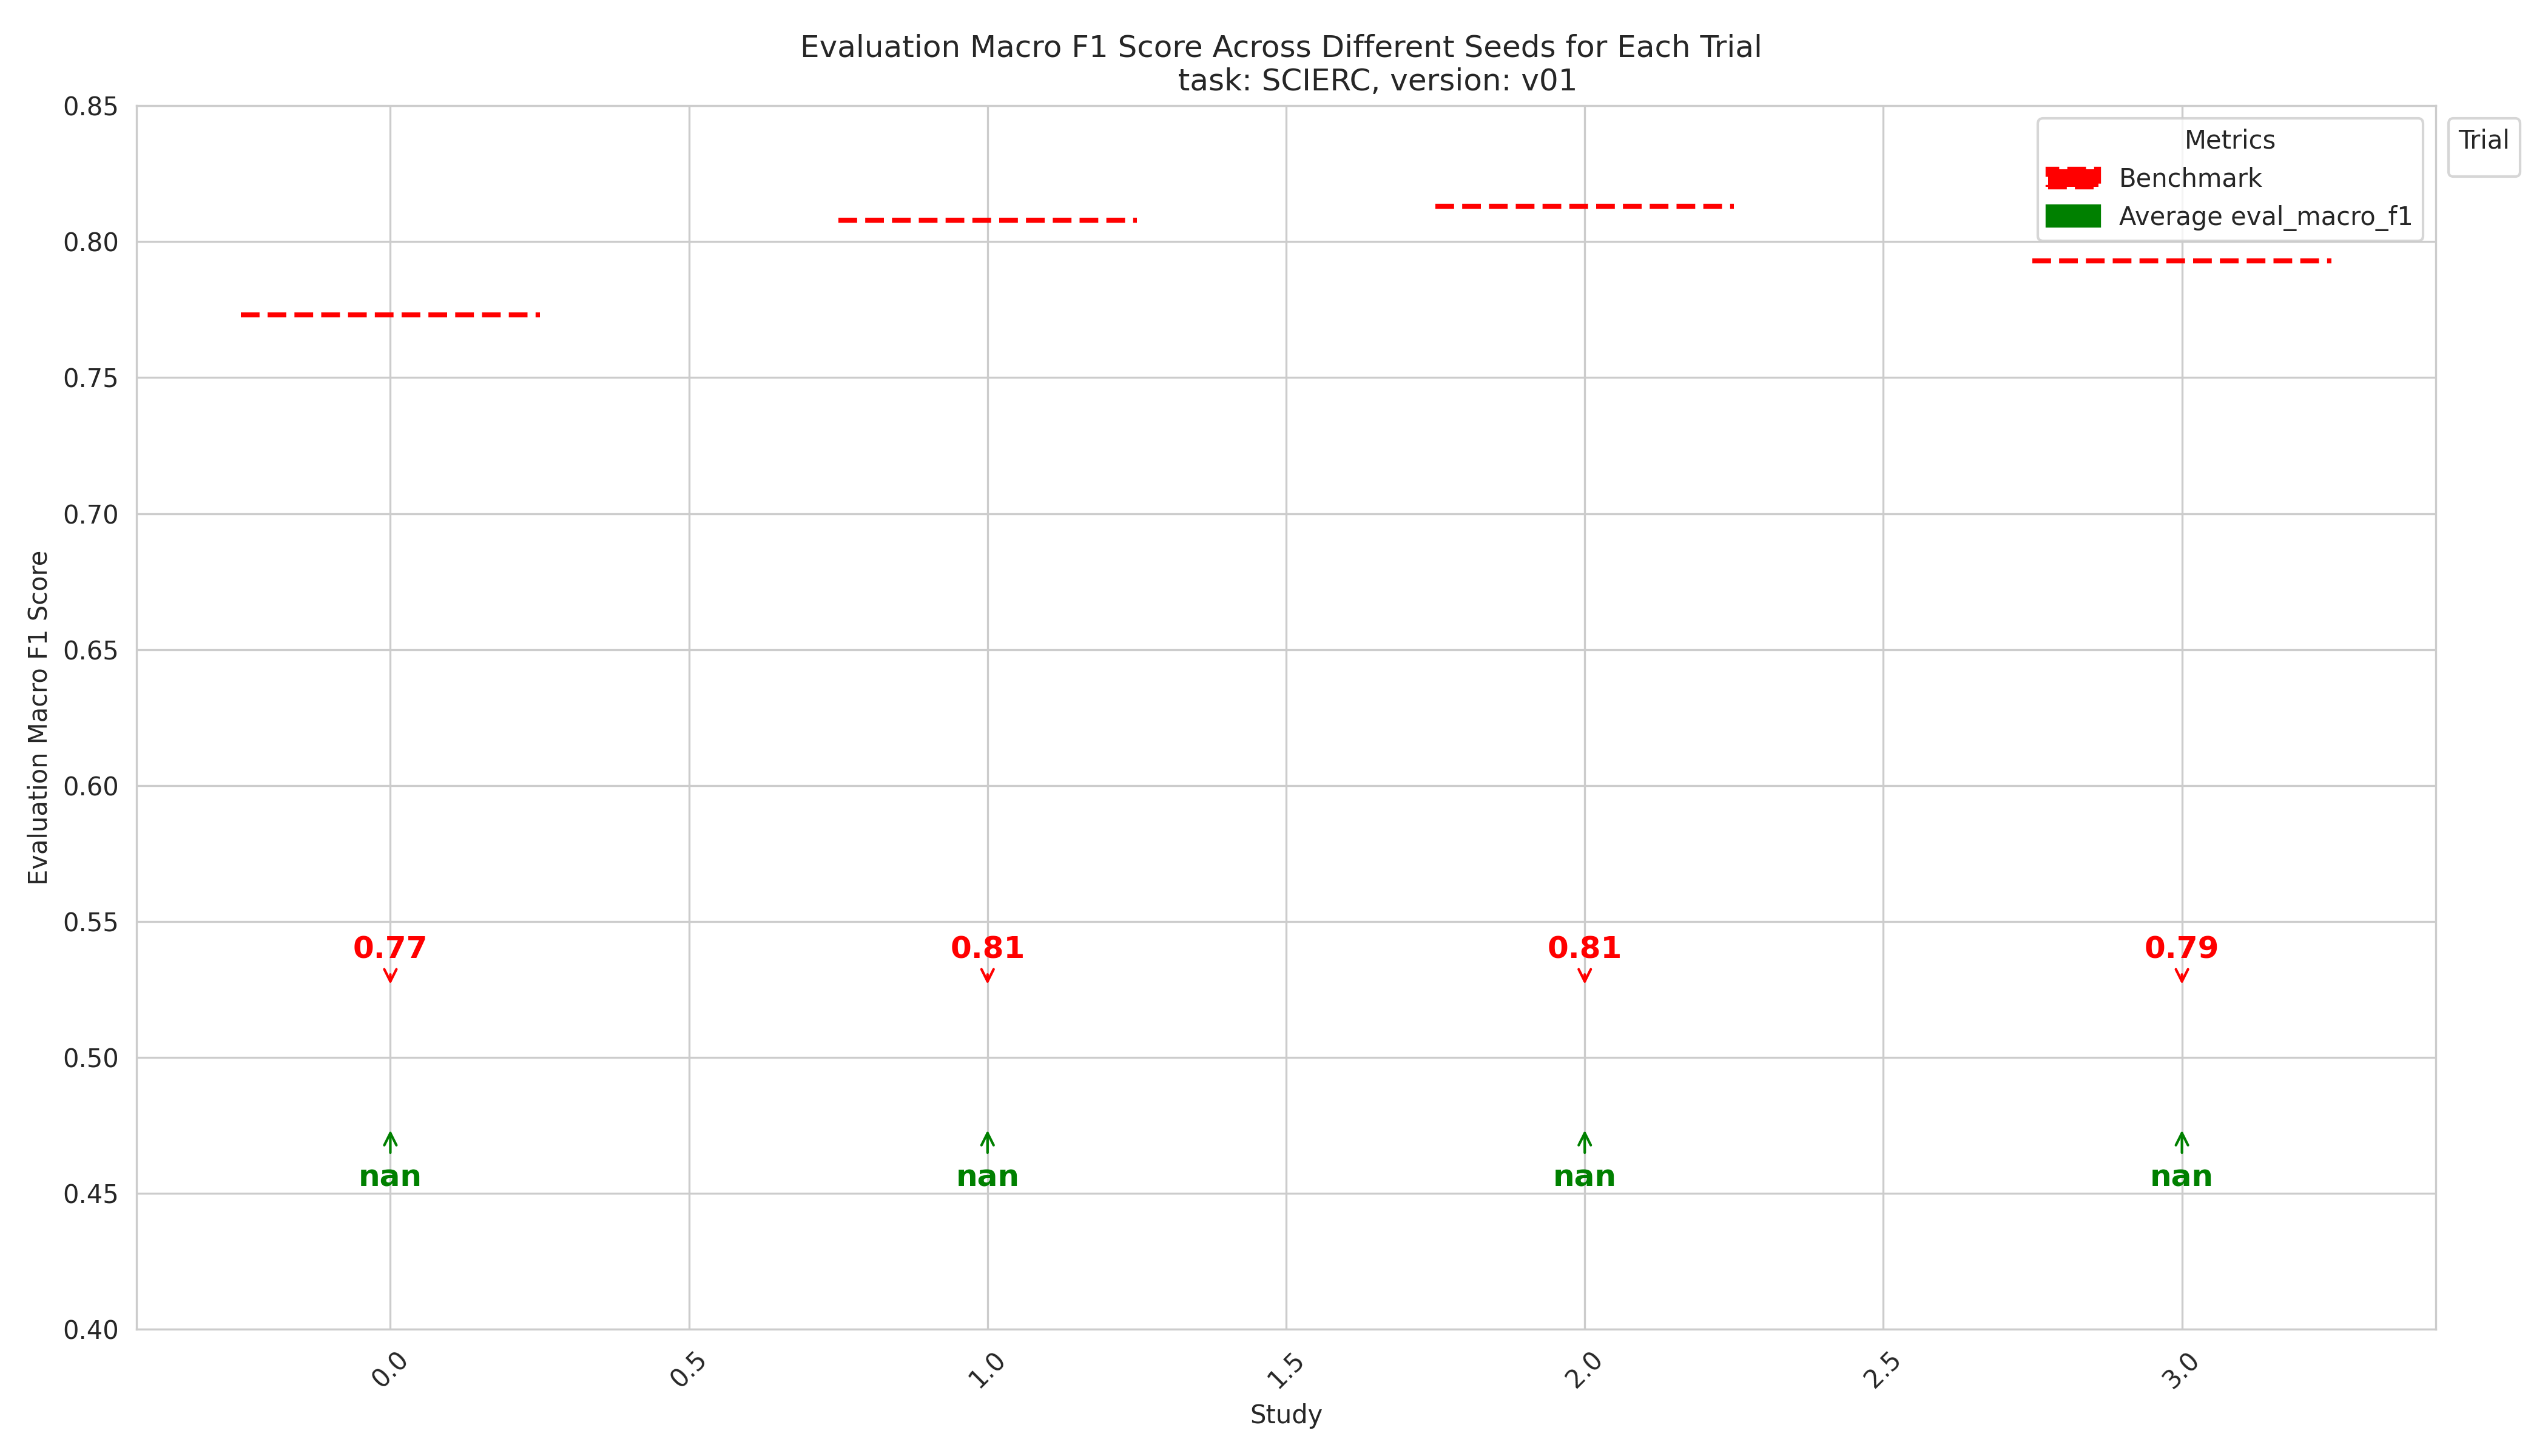
\includegraphics[width=0.45\textwidth]{resources/SCIERC/v01/evaluation_macro_f1_across_seeds.png}
    \caption{Optuna Hyperparameter Search for SCIERC Task}
    \label{fig:optuna_search}
\end{figure}


\subsection{Hyperparameter Search} Optuna was chosen as our hyperparameter optimization framework, especially useful in adapter training to traverse the combinations of learning rates, batch sizes and epochs. The framework proved useful for streamlining the hyperparameter search and selecting the next set-up that would likely lead to an improvement in the F1 performance metric, as showin in \ref{fig:optuna_search}. Each combination runs within a trial, and each trial is composed of 5 random seeds \footnote{The processes we ran also showed a lot of stochasticity across runs. We smoothed out most of the variance by the use of five random seeds, which helped in comparing across different runs. This is in line with \cite{allenai_dont_stop_pretraining} who report high standard deviation in their results, and also follow a 5-seed mean approach.}. The mean F1 on the test dataset is set as a performance metric for each trial, and we report this together with its standard deviation across the seeds. \textcolor{blue}{[TODO -> POINT TO APPENDIX FOR BEST HYPERPARAMETERS FOUND + LIST SEARCH RANGE FOR ADAPTERS]}


\begin{table*}[h]
    \centering
    \label{table:aclarc}
    \begin{tabular}{@{}lcc|cc|c@{}}
    \toprule
    \textbf{Pre-trained Model} & \multicolumn{2}{c|}{Fine-Tuning} & \multicolumn{2}{c}{Adapters} \\
    \cmidrule(lr){2-3} \cmidrule(lr){4-5}
    & Gururangan & Our Baseline & Pfeiffer & Houlsby & \textbf{Adapter Fussion}  \\
    \midrule
    \multicolumn{1}{c}{\textbf{ACL-ARC}} \\
    ROBERTA & 63.00$_{\text{ 5.80}}$ & 66.34$_{\text{ 4.67}}$ & 67.12$_{\text{ 1.85}}$ & 65.53$_{\text{ 1.30}}$ & \textbf{68.46}$_{\text{ 3.43}}$ \\ 
    TAPT & 67.40$_{\text{ 1.80}}$ & \textbf{69.49}$_{\text{ 2.24}}$ & 67.22$_{\text{ 3.92}}$ & 65.12$_{\text{ 1.22}}$ &  \\ 
    DAPT & \underline{75.40}$_{\text{ 2.50}}$ & \textbf{74.65}$_{\text{ 3.33}}$ & 73.32$_{\text{ 1.79}}$ & 74.03$_{\text{ 3.36}}$ & 70.36$_{\text{ 1.87}}$ \\ 
    DAPT\_TAPT & \underline{75.60}$_{\text{ 3.80}}$ & \textbf{74.89}$_{\text{ 2.48}}$ & 73.20$_{\text{ 2.84}}$ & 72.24$_{\text{ 1.55}}$ & -\\ 
    \midrule
    \multicolumn{1}{c}{\textbf{SCIERC}} \\
    ROBERTA & 77.30$_{\text{ 1.90}}$ & 80.02$_{\text{ 1.20}}$ & \textbf{81.60}$_{\text{ 0.42}}$ & 81.32$_{\text{ 0.71}}$ & 79.84$_{\text{ 0.26}}$ \\ 
    TAPT & 79.30$_{\text{ 1.50}}$ & \textbf{80.95}$_{\text{ 0.74}}$ & 80.80$_{\text{ 1.35}}$ & 80.92$_{\text{ 0.76}}$ &  \\ 
    DAPT & 80.80$_{\text{ 1.50}}$ & \textbf{83.08}$_{\text{ 1.16}}$ & 82.48$_{\text{ 0.54}}$ & 82.55$_{\text{ 0.81}}$ & 81.32$_{\text{ 0.46}}$ \\ 
    DAPT\_TAPT & 81.30$_{\text{ 1.80}}$ & 81.55$_{\text{ 0.74}}$ & 81.47$_{\text{ 0.70}}$ & \textbf{88.81}$_{\text{ 0.58}}$ &  \\ 
    \midrule
    \multicolumn{1}{c}{\textbf{CHEMPROT}} \\
    ROBERTA & \underline{81.90}$_{\text{ 0.10}}$ & 80.69$_{\text{ 0.55}}$ & 80.38$_{\text{ 0.52}}$ & \textbf{80.95}$_{\text{ 0.40}}$ &  \\ 
    TAPT & \underline{82.60}$_{\text{ 0.40}}$ & 79.88$_{\text{ 0.66}}$ & \textbf{80.80}$_{\text{ 0.45}}$ & 80.67$_{\text{ 0.65}}$ &  \\ 
    DAPT & \underline{84.20}$_{\text{ 0.20}}$ & 81.72$_{\text{ 0.41}}$ & 81.85$_{\text{ 0.51}}$ & \textbf{82.16}$_{\text{ 0.68}}$ &  \\ 
    DAPT\_TAPT & \underline{84.40}$_{\text{ 0.40}}$ & 81.71$_{\text{ 0.92}}$ & 81.67$_{\text{ 0.39}}$ & \textbf{82.29}$_{\text{ 0.40}}$ &  \\
    \bottomrule
    \end{tabular}
    \caption{\textbf{Comparison of Fine-tuning and Adapter Methods} We show baseline from the original paper \cite{gururangan2020dont} for reference but use our baseline for comparison with other methods. The best results are in bold (where \cite{gururangan2020dont} wins, its underlined). We further add results for Adapter Fussion, that is based on Pfeiffer (?) adapters.}
\end{table*}

\subsection{Hypothesis} 
\textcolor{red}{[DO WE NEED THIS SECTION HERE? THE HYPOTHESIS IS ALREADY STATED IN THE INTRODUCTION AND OTHER PLACES]}
Based on recent research showing the efficacy of adapters at performing on par with fine-tuning approaches \cite{houlsby2019parameter}, we felt confident that we can get comparable results with adapters. Adapters allow for a lot of flexibility with smaller number of trainable parameters, ability to stack multiple adapters onto the same model, and sequential learning on multiple tasks. Further, we were not very sure if our datasets, given their small size, would be able to highlight any differences between the Pfeiffer and Houlsby architectures. Given the higher number of trainable parameters with Houlsby configuration, we expected Houlsby to have a better performance.

\subsection{Optimization} By using Optuna for hyper-parameter optimization, we were able to create better adapter based results. We used the huggingface library transformers and adapters for our training, which use the Adam optimizer (default) with L2 regularization \textcolor{blue}{[POINT TO APPENDIX FOR TRAINING CONFIGS/ETC]}. Since our tasks were all related to classification, cross-entropy loss was used for training. 


\begin{figure}[h]
    \centering 
    \includegraphics[width=0.45\textwidth]{resources/example_learning_curve.png}
    \caption{Example of Learning Curve for Adapters on SCIERC Task}
    \label{fig:learning_curve}
\end{figure}

\section{Experiments and Results}

\textcolor{red}{[DO WE NEED THIS INTRO?]} For our fine-tuning experiments, we add a classifier layer to the pre-trained models and co-train all the pre-trained weights and the classifier with the task data. For our adapters-based experiments, we add the adapters to the pre-trained models and the classification heads. We then train the adapters, which only trains the adapter layers and the final classification heads, without changing any of the pre-trained weights.

\subsection{Results}


Table \ref{tab:model-parameters} shows the total parameter counts of the models when using fine-tuning and the adapters. Note that the Pfeiffer configuration is much more parameter-efficient than the Houlsby configuration, as it introduces fewer layers. A sample of the layers can be found in the appendix \ref{sec:pfeiffermodel} \ref{sec:houlsbymodel}.



\subsection{Adapters vs Fine-Tuning} Based on our empirical results \ref{tab.adaptersvsftresults}, we see that adapters were able to achieve similar performance as full fine-tuning. \textcolor{red}{[suggest to delete] There is some variation attributable to optimal hyper-parameter settings and the limited time and resources we used to conduct these experiments. However,} the results clearly demonstrate \textcolor{blue}{Can we discuss an example or point to a general pattern? i.e., seems that ACL-ARC results are comparable, and for chemprot superior, SCIERC is mixed but certainly a good alternative, with the outlier of DAPT\_TAPT which probably requires further investigation and confirmation} the capacity of adapters to be as effective at transfer learning as full fine-tuning. The comparison of the models \ref{tab:model-parameters} shows that the adapters needed just a fraction of the total parameters (1.71\% and 2.42\%) to be trained to achieve comparable results. While this is a very small sample set, other works have shown similar results \cite{houlsby2019parameter} with adapters and our experiments are in-line with the expectations.


\subsection{Adapters vs Continued Pre-Training} Adapters serve as both a complement to traditional fine-tuning and as a standalone alternative, offering targeted task optimization while reducing computational costs, which is especially beneficial in settings with limited resources.

In addition, from \ref{table:adapters_vs_tapt} we observe that using adapters without additional task-specific pre-training (Adapter (Base)) provided comparable performance to using TAPT. This provides indication that, for some cases, adapters can serve as an alternative to TAPT, possibly due to an ability to infuse task-specific knowledge into the network throught the new layers. This is especially useful for low-resource tasks, where the cost of additional pre-training may not be justified. It's possible that TAPT may not provide as much benefit over adapters since the task-specific terms may not be well-represented in the pre-training corpus. Adapters, however, allow for more targeted adjustments to the model, focusing specifically on the task-relevant aspects of the language without requiring extensive re-training of the model.

The experiments suggest that domain-specific pre-training (DAPT) provides a strong foundation for tasks within that domain, and adapters can effectively leverage and build upon this foundation. Adapters appear to be effective across different sizes of datasets. For smaller datasets, like ACL-ARC and SCIERC, they can provide the necessary specialization without extensive re-training. For larger datasets, such as CHEMPROT, adapters actually improve performance, indicating their utility across different scales of data availability.


\begin{table}[H]
    \centering
    \label{table:adapters_vs_tapt}
    \begin{tabular}{@{}lccccc@{}}
    \hline
    Base PT Model & TAPT & \multicolumn{2}{c}{Adapter} \\
    \cmidrule(lr){2-2} \cmidrule(lr){3-4}
    & & (Base) & (TAPT) \\
    \multicolumn{1}{c}{\textbf{ACL-ARC}} \\
    ROBERTA & \textbf{69.49}$_{\text{ 2.24}}$ & 67.12$_{\text{ 1.85}}$ & 67.22$_{\text{ 3.92}}$ \\
     DAPT & \textbf{74.89}$_{\text{ 2.48}}$ & 74.03*$_{\text{ 3.36}}$ & 74.03*$_{\text{ 3.36}}$ \\
    \hline
    \multicolumn{1}{c}{\textbf{SCIERC}}\\
    ROBERTA & 80.95$_{\text{ 0.74}}$ & \textbf{81.60}$_{\text{ 0.42}}$ & 80.92*$_{\text{ 0.76}}$ \\
    DAPT & 81.55$_{\text{ 0.74}}$ & 82.55*$_{\text{ 0.81}}$ & \textbf{88.81}*$_{\text{ 0.58}}$ \\
    \hline
    \multicolumn{1}{c}{\textbf{CHEMPROT}}\\
    ROBERTA & 79.88$_{\text{ 0.66}}\downarrow$ & \textbf{80.95}*$_{\text{ 0.40}}$ & 80.80$_{\text{ 0.45}}$ \\
    DAPT & 81.71$_{\text{ 0.92}}\downarrow$ & 81.85$_{\text{ 0.51}}$ & \textbf{82.29}*$_{\text{ 0.40}}$ \\
\end{tabular}
\caption{\textbf{Adapters as an alternative to TAPT} The best results are in bold. Note that entries in the matrix that fall for DAPT and TAPT have three phases of pre-training (base, DAPT and TAPT). For Adapters, where it includes a * it refers to Houlsby adapters, otherwise is Pfeiffer. A down arrow$\downarrow$ in TAPT indicates its the lowest score in the row.}
\end{table}


\subsection{Pfeiffer vs Houlsby} Given the higher number of trainable parameters with Houlsby compared to Pfeiffer, we expected Houlsby configuration to perform better than Pfeiffer, in general. While the sample size is small to imply too broad a conclusion, we can see that for the chosen tasks and with the hyper-parameters chosen, the Houlsby configuration was slightly better than Pfeiffer, especially when the dataset is larger. When the datasets are small there is no discernible difference, as both configurations are equally capable of optimal learning. It is expected that Houlsby would be better generally, given the higher number of trained parameters introduced by the Houlsby configuration (2.42\% vs 1.71\%). However, Pfeiffer configuration does have a definite advantage of being more parameter-efficient and this would be a desirable quality when we are talking of lots of tasks. We could see a bit of tradeoff in parameter-efficient configuration vs task performance for bigger datasets.

\subsection{Adapter Composition/Fusion}
TBD




\section{Conclusions}
Through our experiments, we were able to demonstrate the capabilities of adapters to perform at par with fine-tuning alternatives for transfer learning tasks. While needing less than 3\% of the total trainable parameters as compared to fine-tuning, the adapters performance for the tasks matched full fine-tuning.

We also see that the benefits of pre-training across domain and task applied to adapters as well.
Additionally, we also were able to compare the two popular adapter architectures – Pfeiffer and Houlsby. While the Houlsby architecture performed slightly better than the Pfeiffer architecture for our tasks and settings, Pfeiffer architecture was more parameter-efficient and comparable to Houlsby. 

Adapter composition allowed us to create a single model capable of performing multiple tasks using the parameter-efficient adapters. The combined model was at par with the individual adapters for each task since adapters do not suffer from forgetting previous tasks when learning new ones. This has significant benefits for inference, where the same model can perform multiple tasks as well as individual models, while requiring a much smaller size.

Future work could explore additional adapter architectures, composition strategies, and their application across a wider range of NLP tasks and domains.


%-------------------------------------------------------------------------
\onecolumn

\section{Team Members}




Our team was made up of three members. We all participated in periodic zoom calls where we discussed the technical details and work allocation of the project with equal participation from all.

\begin{itemize}
    \item Girish Sharma worked on the initial experiments on fine-tuning and adapters, and later worked on different adapter configurations.
    \item Matias Vizcaino worked on the implementation of the fine-tuning and adapter modules using Optuna on the PACE computers. He also studied the potential of adapters as an alternative to TAPT.
    \item William Gleason worked on the adapter composition and fusion experiments
\end{itemize}

\begin{table*}[h]
\begin{center}
\begin{tabular}{|l|c|p{8cm}|}
\hline
\textbf{Student Name} & \textbf{Contributed Aspects} & \textbf{Details} \\
\hline
Girish Sharma & Implementation and Analysis & Initial fine-tuning and adapter experiments with 5 seeds. Used manual hyper-parameter optimization. Comparison of Pfeiffer and Houlsby adapter architectures.  \\
Matias Vizcaino & Implementation and Analysis & Using Optuna-based hyper-parameter optimization for fine-tuning and adapter experiments. Created final results for fine-tuning and adapters. \\
William Gleason & Implementation and Analysis & Study of adapter composition using Adapter Fusion and other techniques. \\
\hline
\end{tabular}
\end{center}
\caption{\textbf{Contributions of team members.}}
\label{tab:contributions}
\end{table*}
\FloatBarrier


\section{Appendix}
\subsection{Task Dataset Balance}
% Insert a figure that spans both columns
\begin{figure*}[h] % 'h' suggests the figure appears in the specified location
    \centering % Center the image
    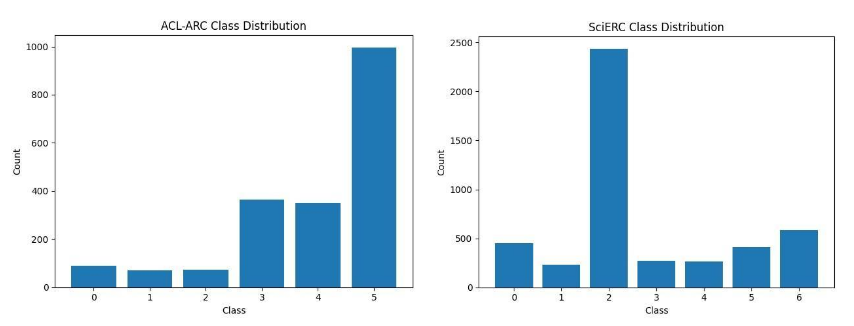
\includegraphics[width=\textwidth]{./resources/DatasetBalance.png} % Make the image full page width
    \caption{Class Distribution for ACL-ARC and SciERC datasets} % Add a caption
    \label{fig:example} % Label the figure for cross-referencing
\end{figure*}
Showing the class distribution for the two tasks in the computer science domain. \ref{fig:example}
\FloatBarrier

\subsection{Model layers}
Layers shown with parameter counts. Only showing the 1st layer for sample purposes. RoBERTa has 11 repeating layers.
\subsubsection{RoBERTa }
\label{sec:robertamodel} 
\textbf{Repeating layers}

roberta.embeddings.LayerNorm.bias: 768

roberta.encoder.layer.0.attention.self.query.weight: 589824

roberta.encoder.layer.0.attention.self.query.bias: 768

roberta.encoder.layer.0.attention.self.key.weight: 589824

roberta.encoder.layer.0.attention.self.key.bias: 768

roberta.encoder.layer.0.attention.self.value.weight: 589824

roberta.encoder.layer.0.attention.self.value.bias: 768

roberta.encoder.layer.0.attention.output.dense.weight: 589824

roberta.encoder.layer.0.attention.output.dense.bias: 768

roberta.encoder.layer.0.attention.output.LayerNorm.weight: 768

roberta.encoder.layer.0.attention.output.LayerNorm.bias: 768

roberta.encoder.layer.0.intermediate.dense.weight: 2359296

roberta.encoder.layer.0.intermediate.dense.bias: 3072

roberta.encoder.layer.0.output.dense.weight: 2359296

roberta.encoder.layer.0.output.dense.bias: 768

roberta.encoder.layer.0.output.LayerNorm.weight: 768

roberta.encoder.layer.0.output.LayerNorm.bias: 768

roberta.encoder.layer.1.attention.self.query.weight: 589824


\textbf{Final Layer}

roberta.encoder.layer.11.output.LayerNorm.bias: 768

classifier.dense.weight: 589824

classifier.dense.bias: 768

classifier.out\_proj.weight: 4608

classifier.out\_proj.bias: 6

\subsubsection{Pfeiffer Adapter}
\label{sec:pfeiffermodel} 
\textbf{Repeating layers}

roberta.embeddings.LayerNorm.bias: 768

roberta.encoder.layer.0.attention.self.query.weight: 589824

roberta.encoder.layer.0.attention.self.query.bias: 768

roberta.encoder.layer.0.attention.self.key.weight: 589824

roberta.encoder.layer.0.attention.self.key.bias: 768

roberta.encoder.layer.0.attention.self.value.weight: 589824

roberta.encoder.layer.0.attention.self.value.bias: 768

roberta.encoder.layer.0.attention.output.dense.weight: 589824

roberta.encoder.layer.0.attention.output.dense.bias: 768

roberta.encoder.layer.0.attention.output.LayerNorm.weight: 768

roberta.encoder.layer.0.attention.output.LayerNorm.bias: 768

roberta.encoder.layer.0.intermediate.dense.weight: 2359296

roberta.encoder.layer.0.intermediate.dense.bias: 3072

roberta.encoder.layer.0.output.dense.weight: 2359296

roberta.encoder.layer.0.output.dense.bias: 768

roberta.encoder.layer.0.output.LayerNorm.weight: 768

roberta.encoder.layer.0.output.LayerNorm.bias: 768

\textbf{roberta.encoder.layer.0.output.adapters.base\_citation\_intent.adapter\_down.0.weight: 36864}

\textbf{roberta.encoder.layer.0.output.adapters.base\_citation\_intent.adapter\_down.0.bias: 48}

\textbf{roberta.encoder.layer.0.output.adapters.base\_citation\_intent.adapter\_up.weight: 36864}

\textbf{roberta.encoder.layer.0.output.adapters.base\_citation\_intent.adapter\_up.bias: 768}

roberta.encoder.layer.1.attention.self.query.weight: 589824

\textbf{Final Layer}

roberta.encoder.layer.11.output.adapters.base\_citation\_intent.adapter\_up.bias: 768

roberta.pooler.dense.weight: 589824

roberta.pooler.dense.bias: 768

\textbf{heads.default.0.weight: 589824}

\textbf{heads.default.0.bias: 768}

\textbf{heads.default.2.weight: 768}

\textbf{heads.default.2.bias: 768}

\textbf{heads.default.3.bias: 50265}

\textbf{heads.base\_citation\_intent.1.weight: 589824}

\textbf{heads.base\_citation\_intent.1.bias: 768}

\textbf{heads.base\_citation\_intent.4.weight: 4608}

\textbf{heads.base\_citation\_intent.4.bias: 6}

\subsubsection{Houlsby Adapter}
\label{sec:houlsbymodel} 

\textbf{Repeating layers}

roberta.embeddings.LayerNorm.bias: 768

roberta.encoder.layer.0.attention.self.query.weight: 589824

roberta.encoder.layer.0.attention.self.query.bias: 768

roberta.encoder.layer.0.attention.self.key.weight: 589824

roberta.encoder.layer.0.attention.self.key.bias: 768

roberta.encoder.layer.0.attention.self.value.weight: 589824

roberta.encoder.layer.0.attention.self.value.bias: 768

roberta.encoder.layer.0.attention.output.dense.weight: 589824

roberta.encoder.layer.0.attention.output.dense.bias: 768

roberta.encoder.layer.0.attention.output.LayerNorm.weight: 768

roberta.encoder.layer.0.attention.output.LayerNorm.bias: 768

\textbf{roberta.encoder.layer.0.attention.output.adapters.base\_citation\_intent.adapter\_down.0.weight: 36864}

\textbf{roberta.encoder.layer.0.attention.output.adapters.base\_citation\_intent.adapter\_down.0.bias: 48}

\textbf{roberta.encoder.layer.0.attention.output.adapters.base\_citation\_intent.adapter\_up.weight: 36864}

\textbf{roberta.encoder.layer.0.attention.output.adapters.base\_citation\_intent.adapter\_up.bias: 768}

roberta.encoder.layer.0.intermediate.dense.weight: 2359296

roberta.encoder.layer.0.intermediate.dense.bias: 3072

roberta.encoder.layer.0.output.dense.weight: 2359296

roberta.encoder.layer.0.output.dense.bias: 768

roberta.encoder.layer.0.output.LayerNorm.weight: 768

roberta.encoder.layer.0.output.LayerNorm.bias: 768

\textbf{roberta.encoder.layer.0.output.adapters.base\_citation\_intent.adapter\_down.0.weight: 36864}

\textbf{roberta.encoder.layer.0.output.adapters.base\_citation\_intent.adapter\_down.0.bias: 48}

\textbf{roberta.encoder.layer.0.output.adapters.base\_citation\_intent.adapter\_up.weight: 36864}

\textbf{roberta.encoder.layer.0.output.adapters.base\_citation\_intent.adapter\_up.bias: 768}

roberta.encoder.layer.1.attention.self.query.weight: 589824

\textbf{Final Layer}

roberta.encoder.layer.11.output.adapters.base\_citation\_intent.adapter\_up.bias: 768

roberta.pooler.dense.weight: 589824

roberta.pooler.dense.bias: 768

\textbf{heads.default.0.weight: 589824}

\textbf{heads.default.0.bias: 768}

\textbf{heads.default.2.weight: 768}

\textbf{heads.default.2.bias: 768}

\textbf{heads.default.3.bias: 50265}

\textbf{heads.base\_citation\_intent.1.weight: 589824}

\textbf{heads.base\_citation\_intent.1.bias: 768}

\textbf{heads.base\_citation\_intent.4.weight: 4608}

\textbf{heads.base\_citation\_intent.4.bias: 6}

\subsection{Models}
The list below shows the pre-trained models used for the two tasks.

task\_models = \{

    \textbf{"citation\_intent"}: \{
    
        "base": "roberta-base",
        
        "dapt": "allenai/cs\_roberta\_base",
        
        "tapt":         "allenai/dsp\_roberta\_base\_tapt\_citation\_intent\_1688",
        
        "dapt\_tapt": allenai/dsp\_roberta\_base\_dapt\_cs\_tapt\_citation\_intent\_1688"
        
    \},

    \textbf{"sciie"}: \{
    
        "base": "roberta-base",
        
        "dapt": "allenai/cs\_roberta\_base",
        
        "tapt": "allenai/dsp\_roberta\_base\_tapt\_sciie\_3219",
        "dapt\_tapt": 
        "allenai/dsp\_roberta\_base\_dapt\_cs\_tapt\_sciie\_3219"
        
    \}
    
\textbf{"chemprot"}: \{

        "base": "roberta-base",
        
        "dapt": " allenai/biomed\_roberta\_base ",
        
        "tapt": " allenai/dsp\_roberta\_base\_tapt\_chemprot\_4169",
        "dapt\_tapt": " 
        allenai/dsp\_roberta\_base\_dapt\_biomed\_tapt\_chemprot\_4169"
        
    \}
    


\section{Source Code}
Source code can be found at the following link:
\href{https://github.gatech.edu/avizcaino3/CS-7643-EfficiencyLane.git}{https://github.gatech.edu/avizcaino3/CS-7643-EfficiencyLane.git}

% {\small
% \bibliographystyle{ieeetr}
% \bibliography{references}
% }

\end{document}
